\documentclass[11pt,a4paper]{article}
\usepackage[utf8]{inputenc}
\usepackage{amsmath,amsfonts,amssymb}
\usepackage{graphicx}
\usepackage{geometry}
\geometry{margin=1in}
\usepackage{booktabs}
\usepackage{hyperref}
\usepackage{float}

\title{\textbf{EE3621: Digital Signal Processing} \\ \Large Lecture 3: The Discrete-Time Fourier Transform (DTFT) \\ \large (III B.Tech EEE)}
\author{Lecture Notes (40-Minute Plan)}
\date{}

\usepackage{xcolor}
\definecolor{darkbg}{HTML}{0d121f}
\definecolor{lighttext}{HTML}{e2e8f0}
\definecolor{primary}{HTML}{8b5cf6}
\definecolor{secondary}{HTML}{0dd5c5}

\pagecolor{darkbg}
\color{lighttext}

\hypersetup{
    colorlinks=true,
    linkcolor=secondary,
    urlcolor=secondary
}

\begin{document}

\maketitle

\section{Lecture Plan \& Objectives (40 Minutes Breakdown)}
\begin{itemize}
    \item \textbf{00:00 -- 05:00 (5 mins):} Motivation: Continuous spectrum for discrete signals and periodic spectrum.
    \item \textbf{05:00 -- 12:00 (7 mins):} DTFT \& IDTFT Definitions and Convergence Criteria.
    \item \textbf{12:00 -- 22:00 (10 mins):} DTFT of Common Signals: Rectangular Pulse, Decaying Exponential, and Double-Sided Exponential.
    \item \textbf{22:00 -- 35:00 (13 mins):} Key Properties of the DTFT with full algebraic proofs.
    \item \textbf{35:00 -- 40:00 (5 mins):} Duality, the Uncertainty Principle, and Checkpoint.
\end{itemize}

\noindent\rule{\textwidth}{0.5pt}

\section{Mathematical Definition of DTFT}
The Discrete-Time Fourier Transform (DTFT) maps a sequence $x[n]$ to a periodic frequency function:
\begin{equation}
X(e^{j\omega}) = \sum_{n=-\infty}^{\infty} x[n] e^{-j\omega n}
\end{equation}
The inverse transform (IDTFT) is:
\begin{equation}
x[n] = \frac{1}{2\pi} \int_{-\pi}^{\pi} X(e^{j\omega}) e^{j\omega n} d\omega
\end{equation}
The DTFT converges uniformly if $x[n]$ is absolutely summable:
\begin{equation}
\sum_{n=-\infty}^{\infty} |x[n]| < \infty
\end{equation}

\section{DTFT of Common Signals}
\subsection{Finite Rectangular Pulse (Length $M$)}
For $x[n] = 1$ for $0 \le n \le M-1$:
\begin{equation}
X(e^{j\omega}) = \sum_{n=0}^{M-1} e^{-j\omega n} = \frac{1 - e^{-j\omega M}}{1 - e^{-j\omega}} = e^{-j\omega(M-1)/2} \frac{\sin(\omega M/2)}{\sin(\omega/2)}
\end{equation}

\subsection{Single-Sided Decaying Exponential}
For $x[n] = a^n u[n]$ ($|a| < 1$):
\begin{equation}
X(e^{j\omega}) = \sum_{n=0}^{\infty} (a e^{-j\omega})^n = \frac{1}{1 - a e^{-j\omega}}
\end{equation}

\subsection{Double-Sided Decaying Exponential}
For $x[n] = a^{|n|}$ ($|a| < 1$):
\begin{equation}
X(e^{j\omega}) = \sum_{n=-\infty}^{-1} a^{-n} e^{-j\omega n} + \sum_{n=0}^{\infty} a^n e^{-j\omega n} = \frac{1 - a^2}{1 + a^2 - 2a\cos\omega}
\end{equation}

\section{Key Properties of the DTFT}
For $x[n] \leftrightarrow X(e^{j\omega})$ and $y[n] \leftrightarrow Y(e^{j\omega})$:

\subsection{Time Shifting}
\begin{equation}
x[n - n_0] \longleftrightarrow X(e^{j\omega}) e^{-j\omega n_0}
\end{equation}
\textit{Proof:} Let $m = n - n_0$.
\begin{equation}
\text{DTFT}\{x[n-n_0]\} = \sum_{n=-\infty}^{\infty} x[n-n_0]e^{-j\omega n} = \sum_{m=-\infty}^{\infty} x[m]e^{-j\omega(m+n_0)} = X(e^{j\omega})e^{-j\omega n_0}
\end{equation}
See Figure~\ref{fig:shifting} for magnitude and phase profiles under time delay.

\begin{figure}[H]
\centering
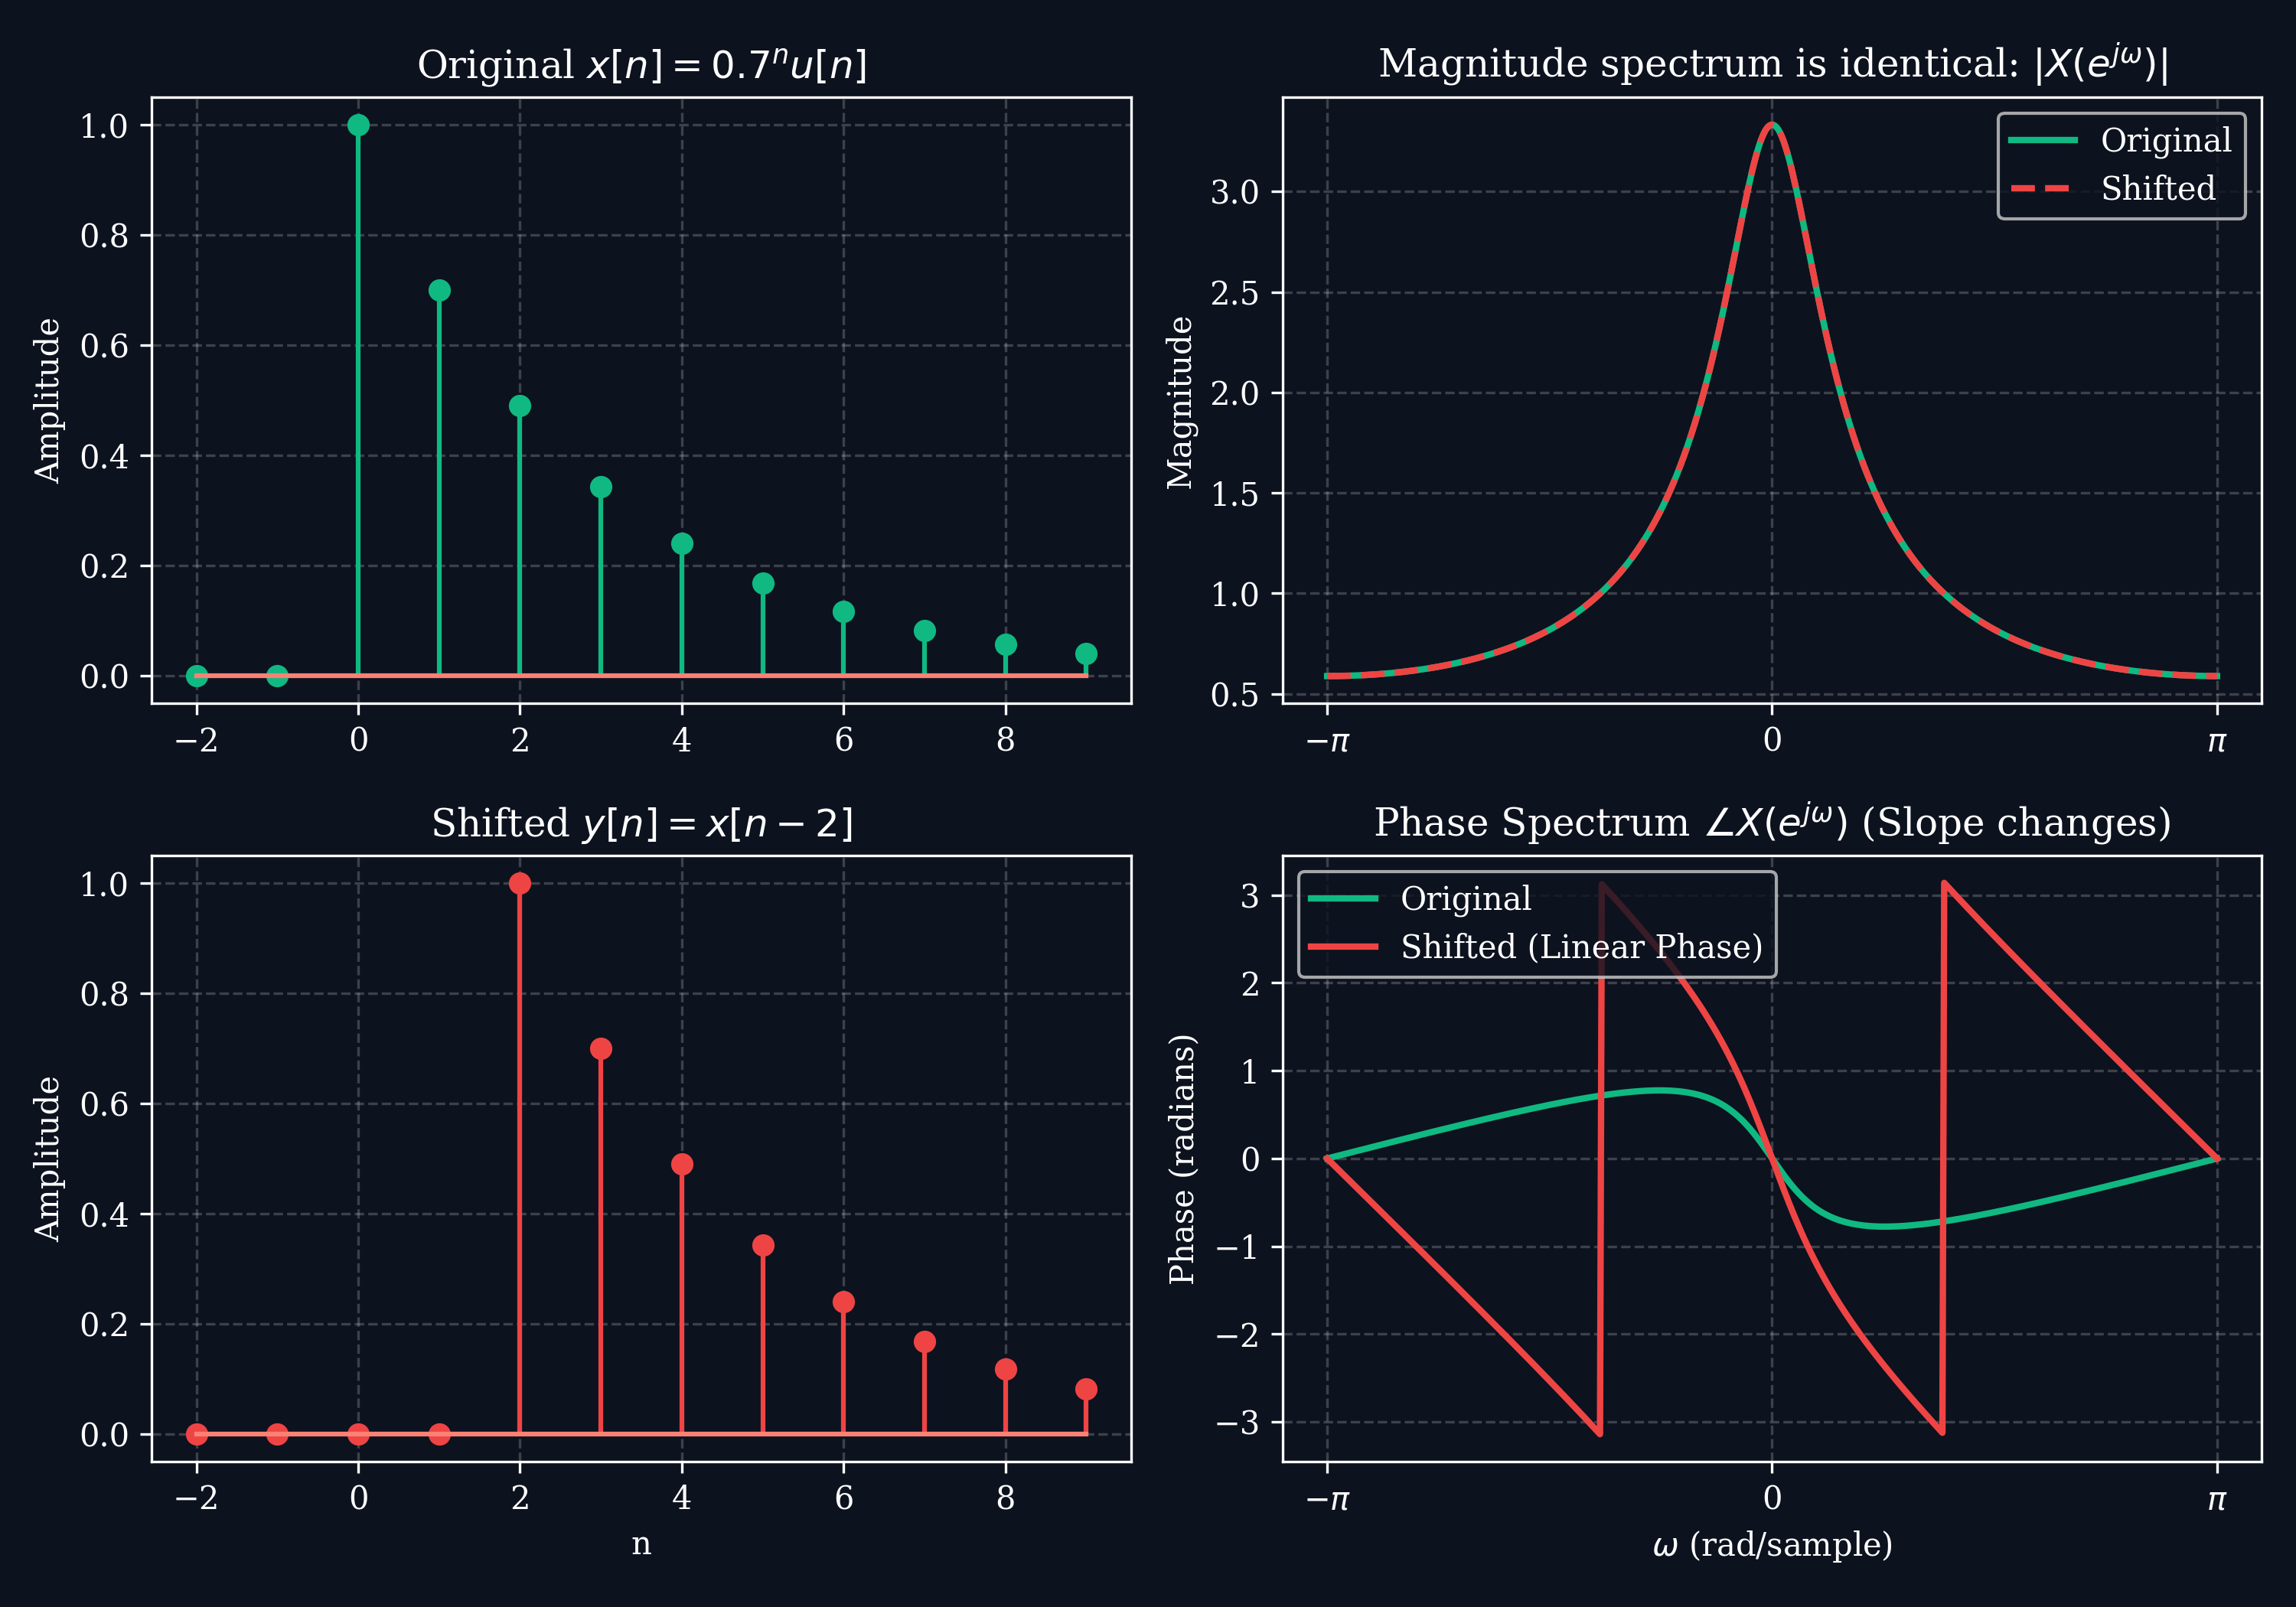
\includegraphics[width=0.85\textwidth]{images/dtft_shifting_property.png}
\caption{Time Shifting property: magnitude response remains invariant while phase shifts linearly.}
\label{fig:shifting}
\end{figure}

\subsection{Frequency Shifting (Modulation)}
\begin{equation}
x[n]e^{j\omega_0 n} \longleftrightarrow X(e^{j(\omega - \omega_0)})
\end{equation}

\subsection{Differentiation in Frequency}
\begin{equation}
n x[n] \longleftrightarrow j \frac{dX(e^{j\omega})}{d\omega}
\end{equation}
\textit{Proof:}
\begin{equation}
\frac{dX(e^{j\omega})}{d\omega} = \sum_{n=-\infty}^{\infty} x[n] (-jn) e^{-j\omega n} \quad \Longrightarrow \quad j \frac{dX(e^{j\omega})}{d\omega} = \sum_{n=-\infty}^{\infty} (n x[n]) e^{-j\omega n}
\end{equation}

\subsection{Convolution Property}
\begin{equation}
x[n] * h[n] \longleftrightarrow X(e^{j\omega}) H(e^{j\omega})
\end{equation}
\textit{Proof:}
\begin{equation}
\sum_{n} (x[n]*h[n]) e^{-j\omega n} = \sum_{n}\sum_{k} x[k]h[n-k]e^{-j\omega n} = \sum_{k} x[k] e^{-j\omega k} \sum_{m} h[m]e^{-j\omega m} = X(e^{j\omega})H(e^{j\omega})
\end{equation}

\subsection{Parseval's Relation}
\begin{equation}
\sum_{n=-\infty}^{\infty} |x[n]|^2 = \frac{1}{2\pi} \int_{-\pi}^{\pi} |X(e^{j\omega})|^2 d\omega
\end{equation}

\section{Duality \& The Uncertainty Principle}
A signal cannot be narrow in both time and frequency domains simultaneously (Figure~\ref{fig:duality}).

\begin{figure}[H]
\centering
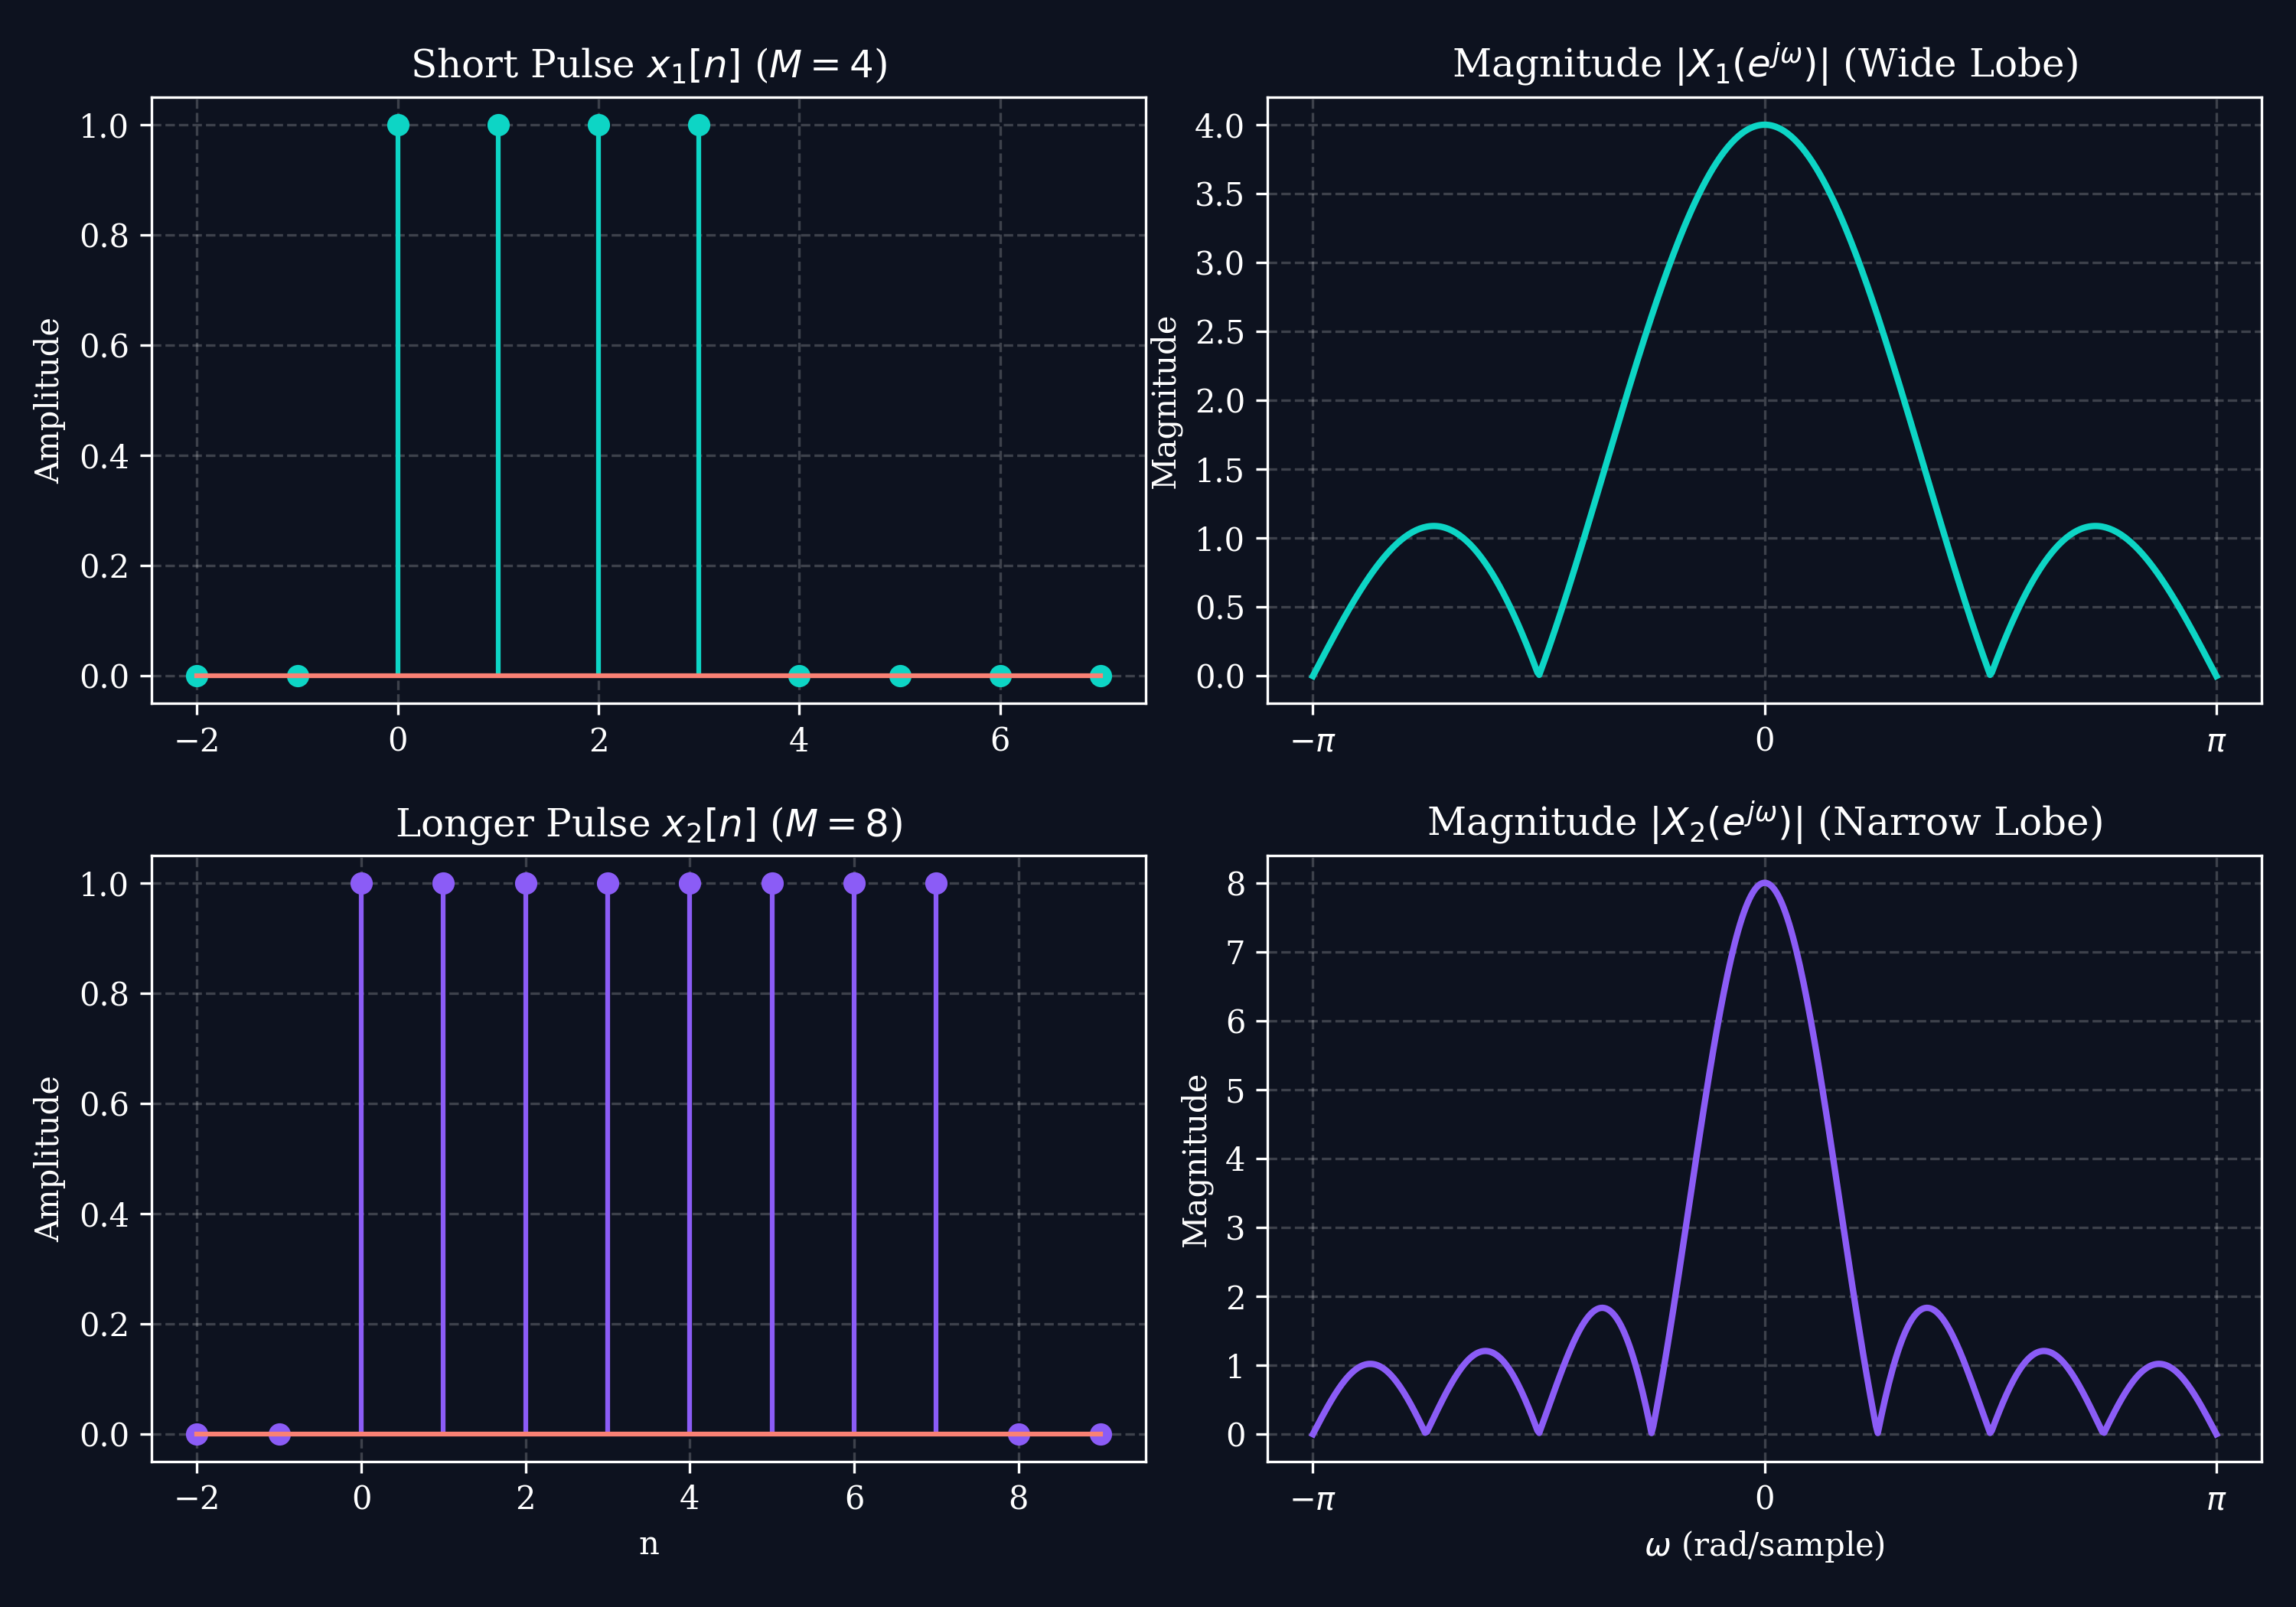
\includegraphics[width=0.85\textwidth]{images/dtft_rect_sinc.png}
\caption{Duality: shorter rectangular time pulse maps to a wider frequency response main lobe.}
\label{fig:duality}
\end{figure}

\end{document}
